%% fcup-thesis.tex -- document template for PhD theses at FCUP
%%
%% Copyright (c) 2015 João Faria <joao.faria@astro.up.pt>
%%
%% This work may be distributed and/or modified under the conditions of
%% the LaTeX Project Public License, either version 1.3c of this license
%% or (at your option) any later version.
%% The latest version of this license is in
%%     http://www.latex-project.org/lppl.txt
%% and version 1.3c or later is part of all distributions of LaTeX
%% version 2005/12/01 or later.
%%
%% This work has the LPPL maintenance status "maintained".
%%
%% The Current Maintainer of this work is
%% João Faria <joao.faria@astro.up.pt>.
%%
%% This work consists of the files listed in the accompanying README.

%% SUMMARY OF FEATURES:
%%
%% All environments, commands, and options provided by the `ut-thesis'
%% class will be described below, at the point where they should appear
%% in the document.  See the file `ut-thesis.cls' for more details.
%%
%% To explicitly set the pagestyle of any blank page inserted with
%% \cleardoublepage, use one of \clearemptydoublepage,
%% \clearplaindoublepage, \clearthesisdoublepage, or
%% \clearstandarddoublepage (to use the style currently in effect).
%%
%% For single-spaced quotes or quotations, use the `longquote' and
%% `longquotation' environments.


%%%%%%%%%%%%         PREAMBLE         %%%%%%%%%%%%

%%  - Default settings format a final copy (single-sided, normal
%%    margins, one-and-a-half-spaced with single-spaced notes).
%%  - For a rough copy (double-sided, normal margins, double-spaced,
%%    with the word "DRAFT" printed at each corner of every page), use
%%    the `draft' option.
%%  - The default global line spacing can be changed with one of the
%%    options `singlespaced', `onehalfspaced', or `doublespaced'.
%%  - Footnotes and marginal notes are all single-spaced by default, but
%%    can be made to have the same spacing as the rest of the document
%%    by using the option `standardspacednotes'.
%%  - The size of the margins can be changed with one of the options:
%%     . `narrowmargins' (1 1/4" left, 3/4" others),
%%     . `normalmargins' (1 1/4" left, 1" others),
%%     . `widemargins' (1 1/4" all),
%%     . `extrawidemargins' (1 1/2" all).
%%  - The pagestyle of "cleared" pages (empty pages inserted in
%%    two-sided documents to put the next page on the right-hand side)
%%    can be set with one of the options `cleardoublepagestyleempty',
%%    `cleardoublepagestyleplain', or `cleardoublepagestylestandard'.
%%  - Any other standard option for the `report' document arclass can be
%%    used to override the default or draft settings (such as `10pt',
%%    `11pt', `12pt'), and standard LaTeX packages can be used to
%%    further customize the layout and/or formatting of the document.

%% *** Add any desired options. ***
%PDF
%\documentclass[a4,narrowmargins,12pt,oneside,draft,onehalfspaced,singlespacednotes]{fcup-thesis}
%\documentclass[a4,narrowmargins,12pt,oneside,onehalfspaced,singlespacednotes]{fcup-thesis}
%Print
%\documentclass[draft,a4,narrowmargins,12pt,twoside,openright,onehalfspaced,singlespacednotes]{fcup-thesis}
\documentclass[a4,narrowmargins,12pt,twoside,openright,onehalfspaced,singlespacednotes]{fcup-thesis}

%% *** Add \usepackage declarations here. ***
%% The standard packages `geometry' and `setspace' are already loaded by
%% `ut-thesis' -- see their documentation for details of the features
%% they provide.  In particular, you may use the \geometry command here
%% to adjust the margins if none of the ut-thesis options are suitable
%% (see the `geometry' package for details).  You may also use the
%% \setstretch command to set the line spacing to a value other than
%% single, one-and-a-half, or double spaced (see the `setspace' package
%% for details).
% Overfull statements
\pretolerance=150
\setlength{\emergencystretch}{3em}
% Overfull end
\usepackage[english]{babel}
\usepackage{lipsum}
\usepackage[utf8]{inputenc}


%%% Additional useful packages
%%% ----------------------------------------------------------------
\usepackage{array}
\usepackage{amsmath}  
\usepackage{amssymb}
\usepackage{amsfonts}
\DeclareFontFamily{OT1}{pzc}{}
\DeclareFontShape{OT1}{pzc}{m}{it}{<-> s * [0.900] pzcmi7t}{}
\DeclareMathAlphabet{\mathpzc}{OT1}{pzc}{m}{it}
\usepackage{amsthm}      
\usepackage[ruled,algochapter]{algorithm2e}
\usepackage{algorithmic}
\usepackage{bm}
\usepackage[mathscr]{euscript}
\usepackage{graphicx}       
\usepackage{psfrag}         
\usepackage{fancyvrb}    
\usepackage{float}
\usepackage{ltablex}
\usepackage[square,sort,comma,numbers]{natbib}        
\usepackage{bbding}         
\usepackage{dcolumn}        
\usepackage{booktabs} 
\usepackage{multirow}
\usepackage{paralist}     
\usepackage{ifdraft}  
\usepackage{indentfirst}    
\usepackage[nottoc,notlof,notlot]{tocbibind}
\usepackage{url}
\usepackage{tabularx}
\usepackage{subcaption}
\usepackage[unicode]{hyperref}
\usepackage{xcolor}

\hypersetup{pdftitle=LiDAR obstacle detection and avoidance, 
            pdfauthor=Alojz Gomola,
            colorlinks=false,
            urlcolor=blue,
            pdfstartview=FitH,
            pdfpagemode=UseOutlines,
            pdfnewwindow,
            breaklinks
          }
\usepackage{array}
\newcolumntype{L}[1]{>{\raggedright\let\newline\\\arraybackslash\hspace{0pt}}m{#1}}
\newcolumntype{C}[1]{>{\centering\let\newline\\\arraybackslash\hspace{0pt}}m{#1}}
\newcolumntype{R}[1]{>{\raggedleft\let\newline\\\arraybackslash\hspace{0pt}}m{#1}}         
\newcolumntype{B}{X}
\newcolumntype{S}[1]{>{\hsize=#1\textwidth}X}

\newcommand{\FIGDIR}{./Pics}    %%% directory containing figures
\newcommand{\twolinecellr}[2][r]{%
  \begin{tabular}[#1]{@{}r@{}}#2\end{tabular}}
\newcommand{\secState}[1]{
	\ifdraft{(#1) }{}
}
\theoremstyle{plain}
\newtheorem{theorem}{Theorem}
\newtheorem{lemma}[theorem]{Lemma}
\newtheorem{proposition}[theorem]{Proposition}

\theoremstyle{plain}
\newtheorem{definition}{Definition}
\newtheorem{problem}{Problem}
\newtheorem{example}{Example}
\newtheorem{assumption}{Assumption}

\theoremstyle{remark}
\newtheorem*{corollary}{Corollary}
\newtheorem*{note}{Note}




\newenvironment{dokaz}{
  \par\medskip\noindent
  \textit{Proof}.
}{
\newline
\rightline{\SquareCastShadowBottomRight}
}

\newenvironment{constraints}[1]{
  \par\medskip\noindent
  \textit{Constraints #1} \\
}{
\newline
\rightline{\SquareCastShadowBottomRight}
}


%\bibliographystyle{plainnat}     %% Author (year) style
\bibliographystyle{unsrt}        %% [number] style
\setcitestyle{square}

% Section  3.7 Challenge list
\newif\ifproblemchallenge   %# Build block for problem challenges
\problemchallengetrue       %# Show comments

\newcommand{\R}{\mathbb{R}}
\newcommand{\N}{\mathbb{N}}

\DeclareMathOperator{\pr}{\textsf{P}}
\DeclareMathOperator{\E}{\textsf{E}\,}
\DeclareMathOperator{\var}{\textrm{var}}
\DeclareMathOperator{\sd}{\textrm{sd}}


\newcommand{\T}[1]{#1^\top}        

\newcommand{\goto}{\rightarrow}
\newcommand{\gotop}{\stackrel{P}{\longrightarrow}}
\newcommand{\maon}[1]{o(n^{#1})}
\newcommand{\abs}[1]{\left|{#1}\right|}
\newcommand{\dint}{\int_0^\tau\!\!\int_0^\tau}
\newcommand{\isqr}[1]{\frac{1}{\sqrt{#1}}}
\newcommand{\norm}[1]{\left\lVert#1\right\rVert}


\newcommand{\pulrad}[1]{\raisebox{1.5ex}[0pt]{#1}}
\newcommand{\mc}[1]{\multicolumn{1}{c}{#1}}
\newcommand{\TBD}[1]{\color{red}\emph{--TBD:}#1\color{black}}

%%%%%%%%%%%%%%%%%%%%%%%%%%%%%%%%%%%%%%%%%%%%%%%%%%%%%%%%%%%%%%%%%%%%%%%%
%%                                                                    %%
%%                   ***   I M P O R T A N T   ***                    %%
%%                                                                    %%
%%  Fill in the following fields with the required information:       %%
%%   - \degree{...}       name of the degree obtained                 %%
%%   - \department{...}   name of the graduate department             %%
%%   - \gradyear{...}     year of graduation                          %%
%%   - \author{...}       name of the author                          %%
%%   - \title{...}        title of the thesis                         %%
%%%%%%%%%%%%%%%%%%%%%%%%%%%%%%%%%%%%%%%%%%%%%%%%%%%%%%%%%%%%%%%%%%%%%%%%

%% *** Change this example to appropriate values. ***
\degree{Doctor of Philosophy}
\department{Departamento de Matem\'{a}tica}
\gradyear{2019}
\author{Alojz Gomola}
\title{Obstacle Avoidance Framework based on Reach Sets}

%% *** NOTE ***
%% Put here all other formatting commands that belong in the preamble.
%% In particular, you should put all of your \newcommand's,
%% \newenvironment's, \newtheorem's, etc. (in other words, all the
%% global definitions that you will need throughout your thesis) in a
%% separate file and use "\input{filename}" to input it here.


%% *** Adjust the following settings as desired. ***

%% List only down to subsections in the table of contents;
%% 0=chapter, 1=section, 2=subsection, 3=subsubsection, etc.
\setcounter{tocdepth}{3}

%% Make each page fill up the entire page.
\flushbottom


%%%%%%%%%%%%      MAIN  DOCUMENT      %%%%%%%%%%%%

\begin{document}




%%%%%%%%%%%%%%%%%%%%%%%%%%%%%%%%%%%%%%%%%%%%%%%%%%%%%%%%%%%%%%%%%%%%%%%%
%%  Put your Chapters here; the easiest way to do this is to keep     %%
%%  each chapter in a separate file and `\include' all the files.     %%
%%  Each chapter file should start with "\chapter{ChapterName}".      %%
%%  Note that using `\include' instead of `\input' will make each     %%
%%  chapter start on a new page, and allow you to format only parts   %%
%%  of your thesis at a time by using `\includeonly'.                 %%
%%%%%%%%%%%%%%%%%%%%%%%%%%%%%%%%%%%%%%%%%%%%%%%%%%%%%%%%%%%%%%%%%%%%%%%%

%% *** Include chapter files here. ***
\setcounter{chapter}{2}
%03-Background theory
    \cleardoublepage
\chapter{Background Theory}\label{ch:backGroundTheory}

\paragraph{Motivation:} Cooperative and Non-Cooperative \emph{Sense and Avoid} (SAA) systems are key enablers for the \emph{Unmanned Aerial Systems} (UAS) to routinely access non-segregated airspace \cite{spriesterbach2013unmanned}. Both cooperative and non-cooperative SAA systems are being developed to address this integration requirement.

The \emph{DAA capability} is defined as the automatic detection of possible conflicts by the UAS platform under consideration and performing avoidance maneuvers to prevent the identified collisions. An analysis of the available DAA candidate technologies and the associated sensors for both cooperative and non-cooperative SAA systems is presented in \cite{muraru2011critical}. 

Non-cooperative \emph{Collision Detection and Resolution} (CD\&R) for UAS is considered as one of the major challenges that need to be addressed \cite{lai2012see} for the insertion of UAVs in non-segregated air space. As a result, many non-cooperative sensors for the SAA system have been adopted. Light Detection and Ranging (LIDAR)is used for detecting, warning and avoiding obstacles for low-level flying \cite{sabatini2014lidar}.

An approach to the definition of encounter models and their applications to SAA strategies is presented in \cite{kochenderfer2008encounter} for both cooperative and non-cooperative scenarios.

Since 2014, there is a visible strong political support for developing rules on drones, but regulations are harmonizing slowly. The European Aviation Safety Agency (EASA) has been tasked to develop a regulatory framework for drone operations and proposals for the regulation of "low-risk" UAS operations. In achieving this, EASA is working closely with the Joint Authorities for Regulation of Unmanned Systems (JARUS) \cite{jarus2016regulations}.

\paragraph{Background Areas:} Following Areas are introduced in this chapter:
\begin{enumerate}
    \item \emph{UAS System Model} (sec. \ref{s:uavMotionModel}) - continuous and discrete mathematical models.
    
    \item \emph{Reach Sets} (sec. \ref{s:ReachSets}) - introduction to representation and calculation methods.
    
    \item \emph{Hybrid Automaton} (sec. \ref{s:HybridAutomaton}) - intuitive definition  of the \emph{hybrid automaton}.
    
    \item \emph{LiDAR} (sec. \ref{sec:LiDARStateOfArt}) - a summary of \emph{LiDAR} technology and terminology introduction.
\end{enumerate}

    \section{(R) UAS System Model}\label{s:uavMotionModel}
\noindent
This section strongly follows \cite{lee2011structure}.

\subsection{Continuous-time systems}\noindent

\noindent Consider a class of systems given by functions:
\begin{equation}
    \begin{aligned}
    State Evolution &: input(time)  \to state(state_0,time) \\
    input(time)&: [0,FinalTime] \to \R^p \\
    input(time)&\in \mathbb{R}^p , state(t) \in \mathbb{R}^n \\
    \end{aligned}
\end{equation}
where $input(time)$ and $state(state_0,time)$ are a sets of continuous-time signals. These are often called continuous-time systems because they operate on continuous-time signals. 

Frequently, such systems can be defined by differential equations that relate the input signal to the output signal.

A prototypical description of a controlled (there is a control input signal) continuous-time system is:
\begin{multline}\label{eq:nonlinearsystem}
    \partial/\partial\text{t state}(time) =\\ f(time,state(time),input(time)), input(time) \in Inputs(time)
\end{multline}
where $f:\mathbb{R}\times\mathbb{R}^n\times\mathbb{R}^p\to\mathbb{R}^n$ satisfies the conditions for existence and uniqueness of the ordinary differential equation and $u$ is our control \cite{butcher1987numerical}.

\subsection{Discrete-time systems}
\noindent
\noindent Consider another class of systems given by functions
\begin{equation}\label{eq:Discretegenericuavmodel}
    \begin{aligned}
    State Evolution:& input(k)  \to state(k), \\
    k \in& \{0, t_s, 2.t_s, 3.t_s, \dots i.t_s\}, i \in \N^+\\
    input(k)\in& \mathbb{R}^p , state(k) \in \mathbb{R}^n\\
    \end{aligned}
\end{equation}
where $input(k)$, $state(k)$ is a set of discrete-time signals. They can be represented by a function $f$ like $f:\{0, t_s, 2.t_s, 3.t_s, \dots i.t_s\} \to \R^n,  i \in \N^+$ where $t_s$ is sampling time and $i$ is discrete step \cite{shampine1997matlab}.

\subsection{Adversarial behaviour in continuous systems}
\noindent Consider a subclass of continuous time systems where are two sets of control signals $uas(time)$ and $adversary(time)$ which are accommodated in following system:
\begin{equation}\label{eq:Adversarial}
    \begin{aligned}
    \partial / \partial \text{t state}(time)&= f(t,state(time),uas(time),adversary(time)), \\
    uas(time) &\in UAS Inputs(time) \subset \R^u, \\
    adversary(time) &\in Adversary Inputs(time) \subset \R^v \\
    \end{aligned}
\end{equation}
This system representation is often used in definition of problem of pursuit/evasion problem. Krasovskii developed a solution approach to this problem in \cite{game1987}. A complex example of can be found in article \cite{game1988}.
    \section{Reach Sets}\label{s:ReachSets}
    \noindent Informally, the \emph{Reach Set} of a UAS system described by a differential equation is the \emph{set of all states that can be reached from an initial state within a given time interval}.

\subsection{Definitions}\label{sec:reachSetIncrementalDefinition}
    \paragraph{For following definitions} consider \emph{nonlinear UAS system} described in (sec. \ref{s:uavMotionModel}).
    
    \begin{definition}[Reach set starting at a given point]\label{def:reachset01}
        Suppose the initial position
        and time $(state_0, time_0)$ are given. The reach set $ReachSet[\tau, time_0, state_0]$ of \emph{nonlinear system} at time $\tau \ge time_0$, starting at $(state_0, time_0)$ is given by:
        \begin{equation}
            ReachSet[\tau, time_0, state_0] = \bigcup \{state(\tau):input(s)\in Inputs(s),s \in (time_0,\tau]\}
        \end{equation}
    \end{definition}
    
    \paragraph{Reach set starting at given set} can be used to determine reach set in case of \emph{hybrid system} input control switch and it is defined as follow:
    \begin{definition}\label{def:ReachSetBasic} set starting at a given set]
        The reach set at time $\tau > t_0$ starting from set $States_0$ is defined as:
        \begin{equation}
            ReachSet[\tau, time_0, States_0] = \bigcup \{ReachSet[\tau, time_0, state_0]: state_0 \in States_0\}
        \end{equation}
    \end{definition}

    \paragraph{Reach set for adversarial behavior} can be used to calculate possible escape routes from pursuer and it is defined as follow:

    \begin{definition}[Reach set under adversarial behavior]
        Consider now the case of adversarial behavior(\cite{game1987,game1988}).
        where $input(t)$ is our control and $adversary(t)$ is adversary control which is independent of $input(t)$, let $differentialControl(t)=input(t)-$ $\sup_{{state} \in state(t)}$\\ $adversary(t)$, which represents worst possible input change in given state and time, then \emph{reach set for system} is represented as:
        \begin{equation}
            ReachSet\left[\begin{gathered}\tau,\\ time_0,\\ state_0\end{gathered}\right] = \bigcup \left\{state(\tau): 
                \begin{aligned}
                    differentialControl(s)\in\\  DifferentialControlSet(s)
                \end{aligned}
            ,s \in (time_0,\tau]\right\}
        \end{equation}
    \end{definition}

    \paragraph{Reach set under constraints} are usable to define state constrained systems in terms of dynamics and technical capabilities.
    
    \begin{definition}[Reach set under state constraints]
        Suppose the initial position and time $(state_0, time_0)$ and $state$ constraints are given $state(t) \in \mathbb{A} \subset \R^n, \dot{x}(t) \in \mathbb{B} \subset \R^n$. The reach set $ReachSet[\tau, time_0, \vec{state}_0]$ of \emph{nonlinear UAS system} at time $\tau \ge time_0$, starting at position and time $(state_0, time_0)$ is given by:
        
        \begin{equation}
            ReachSet\left[\begin{gathered}\tau,\\ time_0,\\ state_0\end{gathered}\right] = \bigcup 
            \left\{
                state(\tau):
                \begin{gathered}
                    \forall s\in (time_0,\tau], state(s) \in \mathbb{A},\\ 
                    \dot{state}(s) \in \mathbb{B},\\ 
                    \exists input(s) \in Inputs(s)
                \end{gathered}
            \right\}
        \end{equation}
        
    \end{definition}


    \subsection{Computation of Reach Sets}
    \noindent   Several techniques for reachability analysis of systems have been proposed. They can be (roughly) classified into two kinds:
    
    \begin{enumerate}
    \item Purely symbolic methods based on: 
        \begin{enumerate}[a.]
        \item the existence of analytic solutions of the differential equations and 
    
        \item the representation of the state space in a decidable theory of the real numbers.
        \end{enumerate}
    \item Methods that combine 
    \begin{enumerate}[a.]
        \item numeric integration of the differential equations
    
        \item symbolic representations of approximations of state space typically using (unions of) polyhedra or ellipsoids.
        \end{enumerate}
    \end{enumerate}
    These techniques provide the algorithmic foundations for the tools that are available for computer-aided verification of hybrid systems (\cite{daws1996tool}, \cite{henzinger1994symbolic}, \cite{henzinger1995hytech}).

    The set-valued Lebesgue integral provides a conceptual tool for the direct computation of the reach set. In what follows we describe techniques from dynamic optimization which are used to compute reach sets for dynamic systems.

    The relation between dynamic optimization and reachability was first observed in \cite{leitmann1982optimality}. A typical problem of optimal control can be formulated as follows:

    \begin{equation}
        \max \left(
        \begin{gathered}
            \int_{initialTime}^{finalTime} cost(time,state(time),contro(time)) \textnormal{d}time + \dots \\ \dots +FinalCost(state(finalTime))\end{gathered}
        \right)
    \end{equation}
    
    \noindent For nonlinear system:
    \begin{equation}
        \dot{state}(t) = f(t,state(t),control(t)), control(t) \in ControlSet(t) \subset \R^p
    \end{equation}
    
    Where $cost$ is given as cost function of time,state and input and $FinalCost$ represents cost functional.
    There are two main techniques to solve this problem: 
    
    \begin{enumerate}
        \item The maximum principle
        
        \item Dynamic programming. The maximum principle gives necessary conditions of optimality. Dynamic programming may be used to derive sufficientconditions of optimality.
    \end{enumerate}

    A good reference on the maximum principle is \cite{pontryagin1962ef}. A less known reference with detailed geometric interpretations is \cite{girsanov2012lectures}. A good reference on dynamic programming is \cite{bardi2008optimal}.
    
    %\section{(W) Space Segmentation}\label{s:spaceSegmentation}
    \emph{To be done here:}
    \begin{itemize}
        \item Polar space segmentation.
        \item local vs global space segmentation.
        \item benefits of uneven space segmentation.
    \end{itemize}
    \newpage
\section{(R) Movement Automaton}\label{sec:MovementAutomatonBackground}

    \noindent\emph{Movement Automaton} is basic interface approach for discretization of \emph{trajectory evolution}  or \emph{control input} for any \emph{continuous or discrete system model}.
    
    \emph{Main function} of \emph{Movement Automaton is} for system given by equation $\dot{state}=f(time,state,input)$ with initial state $state_0$ to generate \emph{reference trajectory} $\hat{state}(t)$ or \emph{control signal} $input(t)$.
    
    Using \emph{Movement Automaton} as \emph{Control Proxy} will provide us with \emph{discrete command chain} interface. This will reduce the \emph{non deterministic} element from \emph{Evasive trajectory} generation, by reducing infinite maneuver set to finite \emph{movement set}.
    
    \emph{Non determinism} of \emph{Avoidance Maneuver} have been discussed as an issue in following works:
    \begin{enumerate}
        \item Newton gradient method for evasive car maneuvers \cite{vsantin2011combined}.
        \item Non-holistic methods for trajectory generation \cite{pin1990autonomous}.
        \item Stochastic approach to elliptic trajectories generation \cite{andrzejak2001epileptic}.
    \end{enumerate}
    
    \emph{Examples} of \emph{Movement Automaton Implementation} as \emph{Control Element} can be mentioned as follows:
    \begin{enumerate}
        \item Control of traffic flow \cite{kuwata2009real}.
        \item Complex air traffic collision situation resolution system  \cite{frazzoli2001robust,frazzoli2000trajectory}.
        \item SAA/DAA capable avoidance system \cite{gomola2017obstacle}.
    \end{enumerate}


    \subsection{Hybrid Automaton}\label{s:HybridAutomaton}
    \noindent First the notion of  \emph{hybrid} automaton  \cite{lazar2006model,borrelli2006mpc,daws1996tool} needs to be introduced:

    \begin{definition}{Hybrid automaton} (\ref{eq:hybridAutomaton}) is given as structure:
        \begin{equation}\label{eq:hybridAutomaton}
        \begin{aligned}
            HybridAutomaton(&States,SystemState,VectorField,\\
                            &DiscreteTransition,ResetMap)
        \end{aligned}
        \end{equation}
    
        \emph{States} ($Q$) is given as set of discrete states, for every time $t\in Domain$ hybrid automaton stays in exactly one of \emph{states}.
    
        \emph{SystemState} ($x$), is given in domain $x\in\R^n,n\in\N^+$, representing the trajectory evolution.
        
        \emph{VectorField} ($f$) (\ref{eq:vectorField}) is bounded to single $State\in States$ and represents local SystemState evolution, when given automaton State is Active.
        
        \begin{equation}\label{eq:vectorField}
            VectorField: State\times SystemState \to SystemState
        \end{equation}
        
        \emph{DiscreteTransition} ($\varphi$) (eq. \ref{eq:discreteTransition}) indicates changes of states in automaton, the changes are triggered by satisfying specific condition given by State and SystemState. 
        
        \begin{equation}\label{eq:discreteTransition}
            DiscreteTransition:State\times SystemState \to State
        \end{equation}
        
        \emph{ResetMap} ($\rho$) (eq. \ref{eq:resetMap}) defines changes of State to some default value, this change is triggered by specific automaton State and SystemState.
        
        \begin{equation}\label{eq:resetMap}
            ResetMap:State\times SystemState \to SystemState
        \end{equation}
    
    \end{definition}

\subsection{Building Blocks}\label{s:MovementAutomatonBuidlingBlocks}
    \begin{definition}{Movement Primitive:}\label{def:MovementPrimitive}\\\emph{States} from \emph{Hybrid automaton} can be taken as \emph{Movements} in \emph{Movement Automaton}. \emph{MovementPrimitive} (eq. \ref{eq:movementPrimitive}) is describing the \emph{Movement} behaviour as transfer function \emph{VectorField} enriched with parameters. 

    \begin{equation}\label{eq:movementPrimitive}
        \begin{aligned}
            &MovementPrimitive(vectorField,minimalDuration,parameters)\\
            &VectorField:SystemState\times parameters \to SystemState
        \end{aligned}
    \end{equation}
    \end{definition}



    \paragraph{Example: }Let say that \emph{UAS} system is given as $\dot{position}=velocity$, then let us have two \emph{MovementPrimitives}:
    
    \begin{enumerate}
        \item \textit{Stay} - $minimalTime=1s$, $parameters=\{\}$, $VectorField:\dot{position}=0$.
        \item \textit{Move} - $minimalTime=1s$, $parameters=\{velocity\}$, $VectorField:\dot{position}=velocity$.
    \end{enumerate}
    
    \paragraph{Trajectory from Movement Primitives:} The \emph{UAS} should \emph{Move} for $5s$ with velocity $10 m/s$, then \emph{Stay} for $10s$, then move for $7s$ with velocity $4 m/s$, with initial position $position_0=0$ and initial time $t_0=1$ The standard approach is to derive transfer function $position = \Theta(\dots)$
    \begin{equation}\label{eq:trajectoryExample}
        position(t)=\Theta(\dots)
        \begin{cases}
            t \in [0,5] &: 10\times t + position(0)\\
            t \in (5,15] &: 0\times (t-5) + position(5)\\
            t \in (15,22]&: 4\times (t-15) + position(15)
        \end{cases}
    \end{equation}

    The \emph{example} given by (eq. \ref{eq:trajectoryExample}) is fairly primitive, but imagine UAS system given by nonlinear dynamics $\dot{x}=f(x,u,t)$ \cite{fossen2011mathematical}. Then defining transfer function for given command chain can be impossible.

    \begin{definition}{Movement Transition:}\label{def:movementTransition}\\
        \emph{System state} can be different than intended movement application, the notion of \emph{Transition} is therefore introduced as stabilizing element in movement chaining (eq. \ref{eq:movementTransition}).
        \begin{equation}\label{eq:movementTransition}
            Transition:MovementPrimitive\times SystemState \to MovementPrimitive    
        \end{equation}
    \end{definition}

    \paragraph{Trajectory with Transitions:} Introducing two transitions $Transition(Move,Stay)$ and $Transition(Stay,Move)$ reflecting periods when vehicle stop moving or speed-up to desired velocity. The transfer function (eq. \ref{eq:trajectoryExample}) can be rewritten as combination of \emph{MovementPrimitives} (eq. \ref{eq:movementPrimitive}) and \emph{Transitions} (eq. \ref{eq:movementTransition}):
    
    \begin{multline}
        Transition(Stay,Move), Move(5s,10m/s),\\
        Transition(Move,Stay), Stay(10s),\\ 
        Transition(Stay,Move), Move(7s,4m/s)
    \end{multline}.

    \begin{note} There are two types of \emph{MovementPrimitives}:
    \begin{enumerate}
        \item \emph{Stationary} - when system state is considered neutral and they are considered as entry point for automaton.
        \item \emph{Dynamic} - when the system state is considered evolving and they needs to be terminated with \emph{stationary} transition.
    \end{enumerate}
    \end{note}

    \paragraph{Movement Mapping Example:} Transition/MovementPrimitive pairs (eq. \ref{eq:movementTransition}) can be mapped into movements (eq. \ref{eq:movementMappingExample}).
    
    \begin{equation}\label{eq:movementMappingExample}
    \begin{aligned}
        Move(5s,10m/s) &:Transition(Stay,Move), Move(5s,10m/s),\\
        Stay(10s) &: Transition(Move,Stay), Stay(10s),\\ 
        Move(7s,4m/s) &: Transition(Stay,Move), Move(7s,4m/s)
    \end{aligned}    
    \end{equation}

    \begin{definition}{Movement:}\label{def:Movement}\\
        Movement can consist from multiple \emph{Transitions} (eq. \ref{eq:movementTransition}) and one \emph{MovementPrimitive} (eq. \ref{eq:movementPrimitive}), the duration of \emph{MovementPrimitive} can be shortened by \emph{Transitions} duration. \emph{Movement} is defined as follows:
        
        \begin{equation}
            \small Movement \left(
                \begin{gathered}
                    \scriptstyle initialState,\\
                    \scriptstyle initialTime[0..1],\\ 
                    \scriptstyle duration,\\ 
                    \scriptstyle parameters[0..1]
                \end{gathered}\right)
            = \small Chain \left(
            \begin{gathered}
            \small InitialTransition(\dots)[0..*],\\
            \small MovementPrimitive\left(
            \begin{gathered}
                \scriptstyle transitionState,\\
                \scriptstyle remainingDuration,\\
                \scriptstyle parameters
            \end{gathered}\right)\\
            \small LeaveTransition(\dots)[0..*],\\
            \end{gathered}
            \right)
        \end{equation}
        
        \emph{Chain function} connects multiple \emph{initial Transitions} which are appliead at \emph{initialState} at \emph{initialTime}. Then own \emph{MovementPrimitive} (eq. \ref{eq:movementPrimitive}) is invoked with \emph{transitionnsState}. \emph{Transitions state} is state changed by \emph{Initial Transitions}. After \emph{Movement Primitive} there can be \emph{Leave Transitions Movement}
    \end{definition}

    \paragraph{Minimal Movement Time:} Given by (eq. \ref{eq:minimalMovementTime}) for \emph{movement} is given as sum of \emph{MovementPrimitive} (eq. \ref{eq:movementPrimitive}) minimal time, and \emph{Transition} (eq. \ref{eq:movementTransition}) in/out combined minimal time.
    
    \begin{equation}\label{eq:minimalMovementTime}
        minimalTime(Movement)=
        \begin{aligned}
        &minimalTime(MovementPrimitive) +\\ &\text{max}_{in/out}\left\{time(Transition)\right\}
        \end{aligned}
    \end{equation}

	\newpage    
    \paragraph{Movement Chaining:}\emph{Movements} can be \emph{chained} and applied to initial \emph{system state} to generate \emph{system trajectory}. Example of trajectory is given by (eq. \ref{eq:trajectoryExample}). Movements are reversibly obtained by participation such \emph{trajectory} into \emph{Movement primitives} and \emph{Transitions}. Then sample \emph{Trajectory} for $n\in \N^+$ movements looks like (eq. \ref{eq:movementChaining}).
    \begin{equation}\label{eq:movementChaining}
        \begin{aligned}
        &Trajectory(t_0)=State(t_0)\\
        &Trajectory(t_0,t_1]=Movement_1(Trajectory(t_0),t_0,duration_1,parameters_1)\\
        &Trajectory(t_1,t_2]=Movement_2(Trajectory(t_1),t_1,duration_2,parameters_2)\\
        &Trajectory(t_2,t_3]=Movement_3(Trajectory(t_2),t_2,duration_3,parameters_3)\\
        &\vdots\\
        &Trajectory(t_{n-1},t_n]=Movement_n(Trajectory(t_{n-1}),t_{n-1},duration_n,parameters_n)\\
        \end{aligned}
    \end{equation}

    Given \emph{Trajectory} at time $t_0$ is given as initial \emph{State} of \emph{System}. For time interval $(t_0,t_1)$, which length is equal to $duration_1$, the \emph{State} is given by $Movement_1$ with $parameters_1$ and base time $t_0$. This behaviour continues for movements $2,\dots,n$. 

    \begin{definition}{Movement Buffer:}\label{def:MovementBuffer}\\
        \noindent\emph{Movements} can be chained into \emph{Buffer} with assumption of \emph{continuous movement execution}. \emph{Continuous movement executions} each movement in chain (eq. \ref{eq:movementChaining}) is executed in time interval $\tau_i=(t_{i-1},t_{i}]$ where $i$ is movement order and $\forall$ $Movement_i$ starting time is $t_0$ or $t_{i-1}$ from previous movement. With given assumption \emph{Buffer} is given as (eq. \ref{eq:movementBuffer}) with parameters $t_{i-1},t_{i}$ omitted, due $t_0$ and $duration_i$ dependency.
        
        \begin{equation}\label{eq:movementBuffer}
            Buffer = \left\{Movement_i(duration_i,parameters_i)\right\}i\in\N^+
        \end{equation}
    \end{definition}
    
    \begin{definition}{Movement Automaton Trajectory:}\label{def:MovementAutomatonTrajectory}\\
        Let say system \emph{State}$\in\R^n$ which \emph{Trajectory} is defined by movement chaining (eq. \ref{eq:movementChaining}), applied on some \emph{initial time} $t_0\in\R^+$ and final time $t_f=t_0+\sum_{i=1}^{I}duration_i$, with movements contained in \emph{Buffer} (eq. \ref{eq:movementBuffer}) is given as \emph{Trajectory} (eq. \ref{eq:TrajectoryDefinition}).
        
        \begin{equation}\label{eq:TrajectoryDefinition}
            Trajectory(t_0,State(t_0),Buffer)\text{ or } Trajectory(State_0,Buffer) \text{ if } t_0=0
        \end{equation}
    \end{definition}


    \begin{note}
        The space dimension of \emph{Trajectories} is $\R^{n+1}$ if the space dimension of state \emph{Space} is $R^n$, because \emph{Trajectory space} contains evolution of \emph{Space} in time interval $T[t_0,t_f]$.
        
        The transformation from \emph{transfer function} (eq. \ref{eq:trajectoryExample}) to \emph{trajectory} (eq. \ref{eq:TrajectoryDefinition}) is natural, only set of \emph{Movement primitives} (eq. \ref{eq:movementPrimitive}) and set of \emph{Transitions} (eq. \ref{eq:movementTransition}) is required.
    \end{note}

    \paragraph{State Projection:} \emph{Trajectory} (eq. \ref{eq:TrajectoryDefinition})is naturally evolution of space over time, then there exists \emph{StateProjection} function (eq. \ref{eq:stateprojection}) which returns \emph{State} for specific \emph{Time}.
    
    \begin{equation}\label{eq:stateprojection}
        StateProjection:Trajectory\times Time \to State(Time)
    \end{equation}

\newpage    
\subsection{Definition}\label{s:MovementAutomatonDefinitionAndProperties}

    \begin{definition}\label{def:movementAutomaton}Movement Automaton is given as follow:
    
    \begin{align}   
        \label{eq:madInitialState}
        InitialState&: \in \R^h, h\in \N^+\\
        \label{eq:madSystemdefinition}
        System&: \dot{State}=f(Time,State,Input)\text{ or } vectorField\\
        \label{eq:madMovementPrimitive}
        Primitives &= \left\{MovementPrimitive_i\left(
                                \begin{aligned}
                                &vectorField,\\
                                &minimalDuration,\\
                                &parameters
                                \end{aligned}\right)
                            \right\} i \in \N^+\\
        \label{eq:madTransitions}
        Transitions&= \left\{Transition_j\left(
                                \begin{aligned}
                                    &MovementPrimitive_l,\\
                                    &MovementPrimitive_k
                                \end{aligned}\right)_{k\neq l}\right\} j\in N^+\\
        \label{eq:madMovements}
        Movements&= \left\{Movement_m\left[
                                \begin{aligned}
                                    &Transition_o[0..*],\\
                                    &MovementPrimitive_p\\
                                    &Transition_r[0..*],\\
                                \end{aligned}\right]_{o \neq r}\right\}  m\in N^+\\
        \label{eq:madBuffer}
        Buffer&= \left\{Movement_s(duration_s,parameters_s)\right\} s\in \N^+\\
        \label{eq:madExecuted}
        Executed&= \left\{Movement_s(duration_s,parameters_t)\right\} t\in \N^+\\
        \label{eq:madBuilder}
        Builder&:Movement \times MovementPrimitive \to Movement\\
        \label{eq:madTrajectory}
        Trajectory&:InitialState\times Movement^u \to State \times Time, u\in N^+\\
        \label{eq:madStateProjection}
        StateProjection&:Trajectory\times Time \to State(Time)  
    \end{align}
    
    \noindent \emph{System} (eq. \ref{eq:madSystemdefinition}) is given in form of \emph{differential equations} $\dot{x} = f(t,x,u)$ or \emph{other transformable equivalent}, with \emph{initial state} (eq. \ref{eq:madInitialState}).
    
    \emph{Movements} (eq. \ref{eq:movementChaining}) are defined as sequence of necessary \emph{initial transitions} (eq. \ref{eq:madTransitions}), \emph{movement primitive} (eq. \ref{eq:madMovementPrimitive}), and, \emph{leave transitions} (\ref{eq:madTransitions}).
    
    \emph{Buffer} contains a set of \emph{movement primitives} (eq. \ref{eq:madMovementPrimitive}) to be executed in order to achieve desired goal. \emph{Builder} (eq. \ref{eq:madBuilder}) assures that first \emph{movement primitive} (eq. \ref{eq:movementPrimitive})from \emph{Buffer} (eq. \ref{eq:madBuffer}) is transformed into \emph{next movement} (eq. \ref{eq:madMovements}) based on \emph{current movement} (eq.\ref{eq:madMovements}).
    
    System \emph{trajectory} (eq. \ref{eq:madTrajectory}) is defined in (eq. \ref{eq:TrajectoryDefinition}). \emph{State projection} (eqs. \ref{eq:stateprojection},\ref{eq:madStateProjection}) is giving \emph{State} variable for time $t\in[t_0,t_{max}]$ where $t_max$ is given by:
    \begin{equation}
    t_{max}=t_0+\sum_{i=1,u}Buffer.Movement(i).movementDuration    
    \end{equation}
    \end{definition}
    
    \begin{note}{From Continuous Reach set to Movement Automaton Control Reach Set:}\label{eq:fromContRStoMARS}

\emph{The reach set $R$} (\ref{eq:reachSetExample1}) for system $\partial/\partial \text{t state} =model(state,input)$ with initial state $state_0=state(t_i)$ in time interval $[t_i,t_{i+1}[$  is with existing control strategy $input(t)\in Control Strategy(t)$. The reach set $R(state_0, t_0,t_1)$ where $t_1 > t_0$.
\begin{equation}\label{eq:reachSetExample1}
    R(state_0, t_0,t_1) = \bigcup \left\{state(s):input(s)\in Control Strategy(s), s\in (t_0,t_1]\right\} 
\end{equation}


\noindent\emph{The reach set $\mathscr{R}$} (\ref{eq:reachSetExample2}) of the system under the control of the \emph{movement automation} consist from the set of trajectories $Trajectory(initialState,buffer)$, which are executed in constrained time period $[t_i,t_{i+1}[$.
\begin{multline}\label{eq:reachSetExample2}
     ReachSet(state_0,t_i,t_{i+1})=\\\left\{Trajectory(state_0,buffer):\text{duration}(buffer) \le (t_{i+1}-t_i)\right\}
\end{multline}
\end{note}

\begin{note}{Weak Invariance:}

When the UAS is under the control of the movement automaton  for the obstacle avoidance problem,  by design of the avoidance algorithm, the trajectories of the UAV will not intersect any threat. This means that the controlled system $\partial/\partial \text{t state} =model(state,input)$ is \emph{weakly invariant} with respect to the complement of the threats, and with respect to the free space. A pair $(state, SafeSpace)$, where $\partial/\partial \text{t state} =model(state,input)$ and $SafeSpace$ is a closed set, is weakly invariant if there exist controls such that a trajectory starting inside $State_0\in SafeSpace$ remains inside $State (t)\in SafeSpace$ \cite{blanchini1999set}.
 \end{note}
    \section{(R) LiDAR}\label{sec:LiDARStateOfArt}
\noindent \paragraph{LiDAR(Light Detection And Ranging)} is active form of remote sensing: information is obtained from a signal which is sent from a transmitter and reflected by a target, and detected by a receiver back at the source. Following types of information can be obtained:
\begin{enumerate}
\item \textit{Range to target} - topographic LiDAR or laser altimeter.
\item \textit{Chemical properties of target} - differential absorption LiDAR.
\item \textit{Velocity of target} - Doppler LiDAR.
\end{enumerate}

\noindent Chemical properties of target are out of scope. Velocity of  target seems as interesting property to investigate, but this type of LiDAR is usually used for meteorological measurements of wind currents \cite{martin2011meteorological}. Extended research in LiDAR as obstacle detection sensor has been executed by research group around Sabatini \cite{sabatini2014lidar} and Ramasy \cite{ramasamy2016lidar}. 

LiDAR output is represented as point cloud it is described by following definition.
\begin{definition}[Scanned point and Point-cloud]
Consider viewpoint as origin of $\R^3$ space,  Let  $point \in Planar Coordinates$ be defined as:
    \begin{equation}
        point = [ distance, horizontal^\circ, vertical^\circ, time ]^T
    \end{equation}
    Where $horizontal^\circ$ is horizontal angle from origin, $vertical^\circ$ is vertical angle to origin, and, $time$ is time of retrieval.\\

    \noindent Point-cloud is set of points scanned in small enough time-frame, based on processing raw point data it can have following representations:
    
    \begin{enumerate}
        \item Local point-cloud - position of sensor is used as origin of space and points can be represented in orthogonal or planar representation. 
        
        \item Global point-cloud -global position of sensor is used as reference to calculate global position of points.
    \end{enumerate}
\end{definition}

\paragraph{Point-cloud} is usually addressed as \textit{raw point-cloud} in case if its represented in Local planar coordinates. Other forms of point cloud require further processing and they are not feasible for real-time obstacle detection and avoidance \cite{chen2007airborne}.

\begin{figure}[H]
    
    \begin{subfigure}{0.5\textwidth}
        \centering
        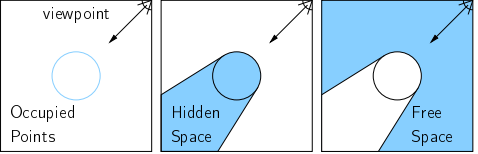
\includegraphics[width=0.9\linewidth]{\FIGDIR/10_Lidar_sets1.PNG} 
        \caption{Space type definitions}
        \label{fig:Spacetypes}
    \end{subfigure}
    \begin{subfigure}{0.5\textwidth}
        \centering
        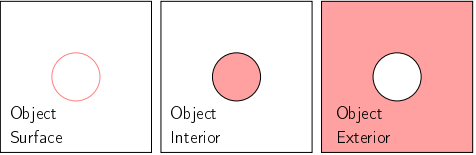
\includegraphics[width=0.9\linewidth]{\FIGDIR/11_Lidar_sets2.PNG}
        \caption{Object properties definitions}
        \label{fig:ObectProperties}
    \end{subfigure}
    
    \caption{Six space classifications \cite{yapo2008probabilistic}.}
    \label{fig:Spaces of interests}
 \end{figure}
 
\noindent  Because of real-time obstacle avoidance it is necessary to introduce following terminology:
\begin{enumerate}
    \item \textit{Occupied points} - points which have been detected by LiDAR (also addressed as visible points).
    \item \textit{Hidden space} - space which is hidden behind occupied points, from viewpoint it is uncertain what is in that space. 
    \item \textit{Free space} - space which is visible from viewpoint and it is not occupied by known objects.
    \item \textit{Object surface} - detected and undetected object surface
    \item \textit{Object interior} - occupied space by object.
    \item \textit{Object exterior} - free space around known objects.
\end{enumerate}

\noindent Existing method for space segregation \cite{yapo2008probabilistic} leads to following definition:

\begin{definition}[Accessible space]\label{def:accessibleSpace}
    Consider known space as space explored by sensor (it can have different viewpoint along previous 3D trajectory).
    Intersection between \textit{object exterior} ($Exterior$) and \textit{free space} $Free$ gives us \textit{Accessible space} ($Accessible$).
    \begin{equation}
        Accessible = Exterior(object) \cap Free(object)
    \end{equation}
\end{definition}
 
 \noindent Accessible space $S_A$ (def. \ref{def:accessibleSpace}) is our bordering limitation for reachable space of system $ReachSet[\tau, time_0, state_0]$ (def. \ref{def:reachset01}.).
    \section{\secState{R}Complementary Definitions}\label{sec:complementsOfAlgebra}

\paragraph{Cartesian Space:} 3D Cartesian space defined by an X, Y, and Z axes (describing position based on horizontal placement, vertical placement, and depth respectively). The coordinates for any point within this space are shown as a vector $[x,y,z]$. \emph{Coordinate system} used this work is the right-handed system (thumbs points at positive direction of x-axis, index finger is pointing to positive direction of y-axis, the positive  of z axis given by remaining fingers).

\paragraph{Base Works:}\emph{Euler} outlined \emph{universal rotation theorem} which was presented in \cite{euler1775formulae}. Rigid body dynamics and rotation matrices defined by Schaub \cite{schaub2003analytical}. 

\paragraph{UAS Coordinate System:} \emph{Local Coordinate frame} is defined by UAS mass center as space center, $Z-$ in direction of gravitational force, $X+$ in direction of UAS heading. This local coordinate system is called Euler Normalized Unit-frame (ENU). 

\paragraph{Rotation Matrices:} Following \emph{Rotation Matrices} are used to transform between two displaced coordinate systems. Roll angle rotation is defined around X-axis by matrix (eq. \ref{eq:rollTransformationMatrix}) on YZ-plane. Pitch angle  rotation matrix is defined around Y-axis by matrix (eq. \ref{eq:pitchTransformationMatrix}) on XZ-plane. Yaw angle rotation matrix is defined around Z axis by matrix (eq. \ref{eq:yawTranformationMatrix}) on XY-plane.

\begin{equation}\label{eq:rollTransformationMatrix}
    R_{YZ} = R_{roll} =
    \begin{bmatrix}
        1 & 0 & 0\\
        0 & \cos(roll) & -\sin(roll)\\
        0 & \sin(roll) & \cos(roll)
    \end{bmatrix}
\end{equation}
\begin{equation}\label{eq:pitchTransformationMatrix}
    R_{XZ} = R_{pitch} =
    \begin{bmatrix}
        \cos(pitch) & 0 & \sin(pitch)\\
        0 & 1 & 0\\
        -\sin(pitch) & 0 & \cos(pitch)
    \end{bmatrix}
\end{equation}
\begin{equation}\label{eq:yawTranformationMatrix}
    R_{XY} = R_{yaw} = 
    \begin{bmatrix}
        \cos(yaw) & -\sin(yaw) & 0 \\
        \sin(yaw) & \cos(yaw) & 1 \\
        0 & 0 & 1
    \end{bmatrix}
\end{equation}
The full rotation matrix in X,Y,Z  is given by (eq. \ref{eq:xyzspaceRotationMatrix}).

\begin{equation}\label{eq:xyzspaceRotationMatrix}  
        R_{XYZ}  = R_{roll,pitch,yaw} =  R_{XY} * R_{XZ} * R_{YZ} = R_{yaw} * R_{pitch} *R_{roll}
\end{equation}

\begin{note}
    The rotation matrix $R_{XYZ}$ (eq. \ref{eq:xyzspaceRotationMatrix}) and its inverse $R_{XYZ}^{-1}$ which gives identity $R_{XYZ} \times R_{XYZ}^{-1} = I$ are used all over this work in transformation.
\end{note}

\paragraph{Gimbal Lock Prevention:} To keep solution numerically stable and rotations numerically stable gimbal lock prevention is necessary \cite{kramer1977gyro}. Gimbal lock occurs when one of matrices (eq. \ref{eq:rollTransformationMatrix}, \ref{eq:pitchTransformationMatrix}, \ref{eq:yawTranformationMatrix}) is singular or final matrix for X,Y,Z rotation is singular (eq. \ref{eq:xyzspaceRotationMatrix}). Gimbal lock leads to loose of one or more degree of freedom, depending on rank and space dimension of singular matrix. To prevent gimbal lock it is necessary to introduce mechanism to check if rotation matrix is regular. For this purpose normative reset function is introduced:
\begin{equation}
    \left [ roll, pitch , yaw \right ]^T = f(t,roll^-,pitch^-,yaw^-), \quad \textnormal{norm}(R_{roll,pitch, yaw})=3
\end{equation}


\noindent Function resets yaw or roll angle to initial position to keep degree of rotation matrix. Simpler but not fault tolerant solution is to keep angles $roll,pitch,yaw \in \left (  -\pi,\pi\right ]$ range.


\paragraph{Polar coordinates:} A \emph{polar coordinate system} represents point in form of vector:
\begin{equation*}
    point_{polar}=[distance, horizontal Dislocation Angle, vertical Dislocation Angle]^T
\end{equation*}
which is ideal for representation of LiDAR scanned point, because usually total point distance and pair of dislocation angles are returned. Using most common LiDAR with horizontal rotation $horizontal^\circ$ and vertical mirror inclination $vertical^\circ$, one can define polar coordinate $point_{polar} = [distance_{x,y,z},horizontal^\circ,vertical^\circ]$ which is dual to Cartesian coordinate $point_{cartesian} = [x,y,z]$. If rotation angle  ranges are $horizontal^\circ,vertical^\circ\in(-\pi,\pi]$ transformation function is bijection.

\paragraph{Polar $\to$ Cartesian:} Transformation from polar to Cartesian representation is defined by following series of functions (eq. \ref{eq:cpt01}, \ref{eq:cpt02},\ref{eq:cpt03}, \ref{eq:cpt04}).

\begin{equation}\label{eq:cpt01}
    distance_{xy} = \cos(horizontal^\circ)\times distance_{xyz}
\end{equation}

\begin{equation}\label{eq:cpt02}
    z = \sin(hirizontal^\circ)\times distance_{xyz}
\end{equation}

\begin{equation}\label{eq:cpt03}
    y = \sin(horizontal^\circ)\times distance_{xy}
\end{equation}

\begin{equation}\label{eq:cpt04}
    x = \cos(vertical^\circ) \times distance_{xy}
\end{equation}


\paragraph{Cartesian $\to$ Polar:} Transformation from Cartesian to polar representation is defined by following series of functions (eq \ref{eq:cpt05}, \ref{eq:cpt06},\ref{eq:cpt07}, \ref{eq:cpt08}).

\begin{equation}\label{eq:cpt05}
    distance_{xyz} = \sqrt{x^2+y^2+z^2}    
\end{equation}

\begin{equation}\label{eq:cpt06}
    distance_{xy} = \sqrt{x^2+y^2}    
\end{equation}

\begin{equation}\label{eq:cpt07}
    horizontal^\circ = \arctan\left(\frac{y}{x}\right)
\end{equation}

\begin{equation}\label{eq:cpt08}
    vertical^\circ =  \arctan \left( \frac{z}{d_{xy}}\right)
\end{equation}

\begin{definition}{Global Coordinate System (GCS) $\mathscr{X}_\mathscr{G}$}\label{def:globalCoordinateSystem}
    takes as center $c_{\mathscr{G}0}$ well known point (for example center of geo-reference model in GNSS systems) every reference distance, plane or angle is calculated taking this center to mind.
\end{definition}

\begin{definition}{Local Coordinate System (LCS) $\mathscr{X}_\mathscr{L}$}\label{def:localCoordinateSystem}
    takes as center $c_{\mathscr{L}0}$ frame of vehicle and can be changing position and orientation in global coordinate frame $\mathscr{X}_\mathscr{G}$.
\end{definition}

\begin{definition}{Global position of polar obstacle $o_i\in\mathscr{O}_{3D}$.}\label{def:globalObstaclePosition3D}
    Let $o_i = [d_o, \theta_o, \varphi_o]^T$ be polar position of obstacle $o_i$ in local coordinate frame of vehicle with global Cartesian position $[x,_v,y_v,z_v]^T$ and normalized orientation angles $[roll_v,pitch_v,yaw_v]$.\\
    Then Cartesian position of obstacle $oi$, $[x_o,y_o,z_o]^T$  in local coordinate frame is given by transformation functions $x_o$ (eq. \ref{eq:cpt04}), $y_o$ (eq. \ref{eq:cpt03}), $z_o$ (eq. \ref{eq:cpt02}).\\ 
    Global  position of polar obstacle $oi$, $[x_g,y_g,z_g]^T$ is given by following equation:
    \begin{equation}
        \begin{bmatrix}
            x_g\\y_g\\z_g
        \end{bmatrix}
        =
        \left [
            R_{XYZ}(roll_v,pitch_v,yaw_v)
            \begin{bmatrix}
                x_o\\y_o\\z_o
            \end{bmatrix}
            +
            \begin{bmatrix}
                x_v\\y_v\\z_v
            \end{bmatrix}
        \right ]
    \end{equation}    
\end{definition}

\begin{definition}{Local position of global coordinate $[x_g,y_g,z_g]^T\in\R^3$.}\label{def:globalToLocal}
    Let there be vehicle with global Cartesian position $[x,_v,y_v,z_v]^T$ and normalized orientation angles $[roll_v,$ $pitch_v,$ $yaw_v]$. in global coordinate frame $\mathscr{X}_\mathscr{X}$.\\
    Then local Cartesian coordinate position $[x_l,y_l,z_l]^T$ of point $[x_g,y_g,z_g]^T$ is given by following equation:
    \begin{equation}
        \begin{bmatrix}
            x_l\\y_l\\z_l
        \end{bmatrix}
        =
        \left [
            R_{XYZ}(-roll_v,-pitch_v,-yaw_v)
            \left (
            \begin{bmatrix}
                x_g\\y_g\\z_g
            \end{bmatrix}
            -
            \begin{bmatrix}
                x_v\\y_v\\z_v
            \end{bmatrix}
            \right )
        \right ]
    \end{equation}
    Local polar position is given as $[distance_l, horizontal_l^\circ,horizontal_l^\circ]$, where $distance_l$ is given by (eq. \ref{eq:cpt05}), $vertical_l^\circ$ is given by (eq. \ref{eq:cpt07}). $vertical_l^\circ$ is given by (eq. \ref{eq:cpt08}), where $[x_l,y_l,z_l]$ are used as local coordinates.
\end{definition}

\paragraph{Polar surface calculation:} The problem is to calculate intersected surface $dA$ of ball subsurface defined by radius $r$, horizontal span $\phi$ and vertical span $\theta$. From classical mechanics one can formulate problem as given by (fig. \ref{fig:80BallSpan}). The intersection plot is in (fig. \ref{fig:81BallSpan2}).

\begin{figure}[H]
    \centering
    \begin{subfigure}[H]{0.3\textwidth}
        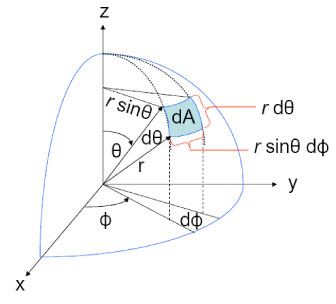
\includegraphics[width=\textwidth]{\FIGDIR/80BallSpan.jpg}
        \caption{Notation}
        \label{fig:80BallSpan}
    \end{subfigure}
    \begin{subfigure}[H]{0.3\textwidth}
        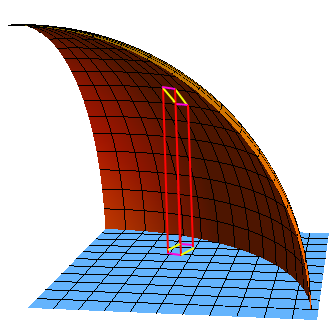
\includegraphics[width=\textwidth]{\FIGDIR/81BallSpan2.png}
        \caption{Plot}
        \label{fig:81BallSpan2}
    \end{subfigure}
    \caption{Polar surface calculation notation and plot}
    \label{fig:BallSpanNOTPLOT}
\end{figure}

\noindent One can use first fundamental form to determine the surface area element. Recall that this is the metric tensor, whose components are obtained by taking the inner product of two tangent vectors in polar space $g_{i,j}= X_i \cdot X_j$, for tangent vectors $X_i$, $X_j$. Following identification for the components of metric tensor will be used:
\begin{equation}\label{eq:metricTensorIdentification}
    g_{ij}=
    \begin{bmatrix}
        E&F\\
        F&G
    \end{bmatrix}
\end{equation}

\noindent Where $E=<X_u,X_u>$, $F=<X_u,X_v>$, and $G=<X_v,X_v>$. Lagrange`s identity can be used , which tells us that the squared area of a parallelogram in space is equal to the sum of the squares of its projections onto the Cartesian plane:
\begin{equation}\label{eq:CartesianProjectionIdentity}
    |X_u \times X_v|^2 = |X_u|^2|X_v|^2 - \left(X_u\cdot X_v\right)^2
\end{equation}

\noindent Given example is displayed in (fig. \ref{fig:81BallSpan2}). The area element is given as:
\begin{equation}\label{eq:squareElementSurfaceDerivation}
    \begin{aligned}
    \text{d}A &= |X_u \times X_v| \quad\text{d}u\text{d}v \\
    & = \sqrt{\left||X_u|^2|X_v|^2 - \left(X_u\cdot X_v\right)^2\right|}\quad \text{d}u\text{d}v\\ 
    & = \sqrt{EG-F^2} \quad \text{d}u\text{d}v
    \end{aligned}
\end{equation}

\noindent We will find tangent vectors via the usual parametrization which give, $X(\phi,\theta)$ = $[r \cos\phi\sin\theta,$ $r\sin\phi\sin\theta,$ $r\cos\theta]$, so that tangent vectors are simply defined as:
\begin{equation}\label{eq:tangentVectorsForPlanarSurface}
    \begin{aligned}
        X_\phi &= [-r\sin\phi\cos\theta,r\cos\phi\sin\theta,0]\\
        X_\theta &=[-r\cos\phi\sin\theta,r\sin\phi\cos\theta,-r\sin\theta]
    \end{aligned}
\end{equation}

\noindent Computing the elements of the first fundamental form gives us:
\begin{equation}
    E = r^2\cos^2\theta,\quad F=0,\quad G=r^2
\end{equation}

\noindent Thus final difference is given as:
\begin{equation}\label{eq:finalCellSquareNice}
    \text{d}A=\sqrt{r^4\cos^2}\quad \text{d}\theta\text{d}\phi = r^2 \cos\theta\quad \text{d}\theta\text{d}\phi
\end{equation}

\begin{note} 
    \emph{Polar Surface} is used in \emph{Detected Obstacle Rating Calculation} (sec. \ref{s:detectedObstacles}). The final formula used in \emph{surface integral calculation} in \emph{non-compact notation} is given as follow:

    \begin{equation}\label{eq:finalCellSquare}
        \text{d}A= r^2 \cos(horizontal^\circ)\quad \text{d}horizontal^\circ \text{d}vertical^\circ
    \end{equation}
\end{note}


	
%% This adds a line for the Bibliography in the Table of Contents.
\addcontentsline{toc}{chapter}{Bibliography}
%% *** Set the bibliography style. ***
%% (change according to your preference/requirements)
%\bibliographystyle{plain}
%% *** Set the bibliography file. ***
%% ("thesis.bib" by default; change as needed)
\bibliography{thesis}

%% *** NOTE ***
%% If you don't use bibliography files, comment out the previous line
%% and use \begin{thebibliography}...\end{thebibliography}.  (In that
%% case, you should probably put the bibliography in a separate file and
%% `\include' or `\input' it here).

\end{document}
